\section{Message Board}
\Writetofile{hints}{\protect\section{Message Board 11}}
\Writetofile{soln}{\protect\newpage\protect\section{Message Board 11}}


\subsection{Problem 1}
$O$ is the circumcenter of the acute triangle $ABC$. The lines $AO, BO, CO$ meet the opposite sides at $D, E, F$ respectively. Show that $\dfrac 1{AD} + \dfrac 1{BE} + \dfrac 1{CF} = \dfrac 2{AO}$.

% https://s3.amazonaws.com/classroom.artofproblemsolving.com/Classes/GeomOlympiad/Images/extcircum.gif
\begin{center}
    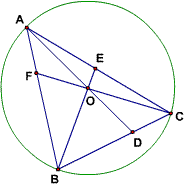
\includegraphics[scale=0.8]{extcircum}
\end{center}

\textit{Has hints.}
\begin{sketch}
    \begin{enumerate}
        \item Construct a perpendicular from A to BC.
        \item Express various ratios in terms of trigonometric functions.
    \end{enumerate}
\end{sketch}

\begin{mdsoln}
    Since $AO=BO=CO=R$, what we want to prove is equivalent to$$\frac{AO}{AD}+\frac{BO}{BE}+\frac{CO}{CF}=2$$But we know that$$\frac{AO}{AD}=\frac{[ACOB]}{[ABC]}$$and similar expressions for $BO/BE$ and $CO/CF$. So$$\frac{AO}{AD}+\frac{BO}{BE}+\frac{CO}{CF}=\frac{[ACOB]+[BAOC]+[CBOA]}{ABC}=2$$as desired.
\end{mdsoln}


\subsection{Problem 2}
Given the following information about a triangle: the radius $R$ of its circumscribed circle, the length $c$ of one of its sides, and the ratio $\dfrac ab$ of the other two sides; determine all three sides and angles of the triangle.

\textit{Has hints.}
\begin{sketch}
    \begin{enumerate}
        \item Use the Law of Sines. (This is good advice in general when you know the circumradius.)
        \item Draw a perpendicular from $C$ to $AB$.
    \end{enumerate}
\end{sketch}

\begin{mdsoln}
    There are actually two possibilities for the triangle: one with $\angle C\ge 90^\circ$ and one with $\angle C\le 90^\circ$ (unless $C=90^\circ$, in which case there is only one possibility). We will find both of these solutions.

    Draw segment $AB$ of length $c$.
    
    We first try to find $D$ on segment $AB$ such that $DB/DA=a/b$ (why we want this will become clear later on). Supposing that we were given $a/b$ as the ratio of some two lengths $x$ and $y$, we can find $D$ in the following manner: Construct a line parallel to and distinct from $AB$ and choose points $X,Y,Z$ on the line such that $XY=x$, $YZ=y$, and $Y$ lies on segment $XZ$. Then, find the intersection $P$ of $XB$ and $ZA$. There is a homothety centered at $P$ taking $X,Y,Z$ to $B,D,A$, respectively, since $BD/DA=XY/YZ$. The desired point $D$ must therefore be the intersection of $PY$ and $AB$.
    
    Now, by the Law of Sines, $\sin \angle C=c/2R$. We construct a circle with diameter $ST$ of length $2R$, and find an intersection point $U$ of the circle with the circle of radius $c$ centered at $S$. It is clear that $\triangle STU$ has a right angle at $U$, that $ST=2R$ and $SU=c$. Hence, $\angle T$ must be equal to angle $\angle C$ or else to $180^\circ-\angle C$. These two possible values for $\angle C$ give us the two solutions to the problem.
    
    For each of the values of $\angle C$, we proceed as follows:
    
    Now we construct points $E,F$ on the same side of line $AB$ such that $AE=DE$, $DF=BF$, and $\angle DEA=\angle BFD=\angle C/2$. The circumcircles of $\triangle ADE$ and $\triangle DBF$ must intersect at some point $Q$ such that $\angle DQA=\angle BQD=\angle C/2$. Hence, $\angle BQA=\angle C$. Moreover, since $QD$ is the angle bisector of $\angle BQA$, the Angle-Bisector Theorem implies that $QB/QA=DB/DA=a/b$. Hence, $Q$ satisfies all the requirements for our desired point $C$.
    
    It is simple to work through this logic to show that our solution does indeed produce all possible solutions to the problem.        
\end{mdsoln}




\subsection{Problem 3}
Show that if $A$, $B$, $C$ are angles of a triangle, then
\[
\sin \dfrac A2 \sin \dfrac B2 \sin \dfrac C2 \leq \dfrac 18.
\]

\begin{mdsoln}
    We proved in class that$$\sin \dfrac A2=\sqrt{\frac{(s-b)(s-c)}{bc}}$$Using this and similar expressions for $\sin (B/2)$ and $\sin (C/2)$, we get\begin{eqnarray*}\sin \dfrac A2 \sin \dfrac B2 \sin \dfrac C2&=&\sqrt {\frac {(s - b)(s - c)}{bc}} \cdot \sqrt {(\frac {(s - c)(s - a)}{ca}} \cdot \sqrt {\frac {(s - a)(s - b)}{ab}}\\ &=& \frac{(s-a)(s-b)(s-c)}{abc}\\ &=&\frac{s(s-a)(s-b)(s-c)}{sabc}\\ &=&\frac{A^2}{sabc}\\ &=&\frac{\frac{abc}{4R}\cdot rs}{sabc}\\ &=&\frac{r}{4R}\\ &\le &\frac{1}{8}\end{eqnarray*}where the last step follows from Euler’s Inequality $R\ge 2r$.
\end{mdsoln}



\subsection{Problem 4}
In triangle $ABC$, prove that there is a point $D$ on side $AB$ such that $CD$ is the geometric mean of $AD$ and $DB$ if and only if
\[
\sin A \cdot \sin B \leq \sin^2 \dfrac C2 .
\]



\textit{Has hints.}
\begin{sketch}
    \begin{enumerate}
        \item Extend $CD$ to the circumcircle of $ABC$.
        \item Use power of a point.
        \item Look for extreme cases.
    \end{enumerate}
\end{sketch}

\begin{mdsoln}
    Suppose that $D$ is just a variable point on side $AB$. Let $P$ be the other intersection of ray $CD$ with the circumcircle $\omega$ of $\triangle ABC$. By Power of a Point, $AD\cdot DB=CD\cdot DP$. Observe that $CD$ is the geometric mean of $AD$ and $DB$ if and only if$$CD^2=AD\cdot DB=CD\cdot DP$$which is the case if and only if $CD=DP$.

    So it suffices to consider whether there exists a $D$ for which $CD=DP$. Consider, for $D$ varying along segment $AB$, the locus $L$ of points $Q$ such that $Q$ is on ray $CD$ with $CD=DQ$. There exists a $D$ such that $CD=DP$ if and only if $L$ intersects $\omega$. Note that $L$ is merely the image of segment $AB$ under a homothety of ratio 2 centered at $C$. $L$ intersects $\omega$ if and only if the tangent line $\ell$ to $\omega$ which is parallel to $AB$ and on the opposite side of it from point $C$ is the image of line $AB$ under a homothety of ratio greater than or equal to 2.
    
    Suppose that $\ell$ is tangent to $\omega$ at $X$. Since $\ell\parallel AB$, $X$ must bisect the arc $AB$, so $CX$ must bisect angle $C$. Let $CX$ meet $AB$ at $Y$. Then, the homothety centered at $C$ taking line $AB$ to $\ell$ has ratio $CX/CY$. Therefore, a $D$ of the desired form exists if and only if $CX/CY\ge 2$, which is equivalent to\begin{eqnarray*}1&\le & \frac{XY}{CY}\\ &=&\frac{XY}{AY}\cdot \frac{AY}{CY}\\ &=&\frac{\sin \angle YAX}{\sin \angle AXY}\cdot \frac{\sin \angle YCA}{\sin \angle CAY}\\ &=&\frac{\sin \angle BCY}{\sin \angle ABC}\cdot \frac{\sin \angle YCA}{\sin \angle CAB}\\ &=&\frac{\sin^2 (C/2)}{\sin B\sin A}\end{eqnarray*}which gives us the desired result.        
\end{mdsoln}





\subsection{Problem 5}
$ABC$ is a triangle. The tangent to the circumcircle at $A$ meets the line $BC$ at $D$. The perpendicular to $BC$ at $B$ meets the perpendicular bisector of $AB$ at $E$, and the perpendicular to BC at C meets the perpendicular bisector of AC at F. Show that D, E, F are collinear.

% https://s3.amazonaws.com/classroom.artofproblemsolving.com/Classes/GeomOlympiad/Images/collfeet.gif
\begin{center}
    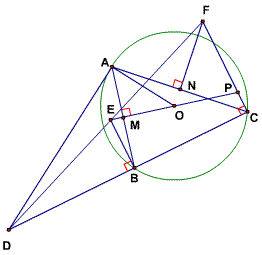
\includegraphics[scale=0.8]{collfeet}
\end{center}

\begin{mdsoln}
    We see that\begin{eqnarray*}FC&=&\frac{\dfrac{1}{2}AC}{\cos(90-\angle C)}\\ EB&=&\frac{\dfrac{1}{2}AB}{\cos(90-\angle B)}\end{eqnarray*}Hence,\begin{eqnarray*}\frac{EB}{FC}&=&\frac{\cos(90-\angle C)}{\cos(90-\angle B)}\cdot \frac{AB}{AC}\\ &=&\frac{\sin\angle C}{\sin\angle B}\cdot \frac{AB}{AC}\\ &=&\frac{\sin\angle BAD}{\sin\angle DBA}\cdot \frac{AB}{AC}\\ &=&\frac{BD}{AD}\cdot \frac{AB}{AC}\\ &=&\frac{BD}{AD\cdot \dfrac{AC}{AB}}\\ &=&\frac{BD}{CD}\end{eqnarray*}where the last step follows from $\triangle ABD\sim \triangle CAD$. Since $EB/FC=BD/CD$, points $D,E,F$ must be collinear, as desired.    
\end{mdsoln}



\subsection{Problem 6}
Given the triangle $ABC$, let $D, E, F$ be the midpoints of $BC, AC, AB$ respectively and $G$ be the centroid of $ABC$. For each value of angle $BAC$, how many non-similar triangles are there in which $AEGF$ is a cyclic quadrilateral.

% https://s3.amazonaws.com/classroom.artofproblemsolving.com/Classes/GeomOlympiad/Images/centro.gif
\begin{center}
    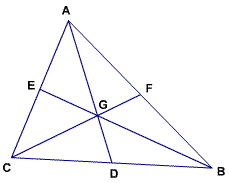
\includegraphics[scale=0.8]{centro}
\end{center}

\begin{mdsoln}
    Fix $\angle BAC$ at some value $\theta$ and fix $BC$ at some value $a$. Clearly, if $AEGF$ is cyclic, then $\angle BGC=180^\circ-\angle BAC$, implying that we need only consider $\theta\le 90^\circ$ (since for $\theta>90^\circ$, angles $BGC$ and $BAC$ are both greater than $90^\circ$, so $AEGF$ cannot be cyclic).

    Observe that $AEGF$ is cyclic implies that $\angle GAE=\angle GFE=\angle GCB$. This implies $\triangle DGC\sim \triangle DCA$, which is in turn implies $CD^2=(DG)(DA)=3DG^2$. Since $CD=a/2$, this means that$$DG=\frac{\sqrt{3}a}{6}$$As previously noted, $AEGF$ cyclic also implies $\angle BGC=180^\circ-\theta$. Hence, $AEGF$ can be cyclic only if (but not necessarily if) both $DG=\dfrac{\sqrt{3}a}{6}$ and $\angle BGC=180^\circ-\theta$. We will now consider how many triangles $BGC$ exist that satisfy both these requirements.
    
    Consider the arc which is the locus of points $G$ such that $\angle BGC=180^\circ-\theta$. The length $GD$ from $G$ to the midpoint $D$ of $BC$ varies from a minimum where $G$ is at the midpoint of the arc (where $GD=(a/2)\cot (\angle BGC/2)=(a/2)\tan(\theta/2)$) to a maximum where $G$ is at either $B$ or $C$ (where $GD=a/2$). The length $GD$ varies continuously between these two extremes. We seek $GD=\frac{\sqrt{3}a}{6}$. If$$\frac{a}{2}\tan(\theta/2)\le \frac{\sqrt{3}a}{6}\le \frac{a}{2}$$then there is either exactly one or exactly two points on the arc with $GD$ as desired (if there are two spots then they yield exactly the same triangle $GBC$, merely reflected about the perpendicular bisector of $BC$). If the inequality above does not hold, then there is no location of $G$ that works, so there are no triangles $ABC$ such that $AEGF$ is cyclic.
    
    We now consider when the inequality holds. Notice that the statement$$\frac{\sqrt{3}a}{6}\le \frac{a}{2}$$is true, and the statement$$\frac{a}{2}\tan(\theta/2)\le =\frac{\sqrt{3}a}{6}$$is true if and only if$$\theta\le 2\tan^{-1}(\frac{\sqrt{3}}{3})=60^\circ$$
    For $\theta\le 60^\circ$, then, there is exactly one triangle $BGC$ that satisfies $DG=\dfrac{\sqrt{3}a}{6}$ and $\angle BGC=180^\circ-\theta$. Letting $A$ be on ray $DG$ such that $DA=3DG$, we see that $G$ must be the centroid of $\triangle ABC$ and that $DG=\dfrac{\sqrt{3}a}{6}$ implies that $\triangle DGC\sim \triangle DCA$ (by our previous logic), so that, if $E$ and $F$ are the midpoints of $AC$ and $AB$, respectively, $\angle GAE=\angle GCB=\angle GFE$. We conclude that $AEGF$ is cyclic and hence that $\angle BAC=180^\circ-\angle BGC=\theta$, so $\triangle ABC$ is a triangle of the desired form.
    
    We conclude that, for $\theta\le 60^\circ$, there is exactly one solution to the problem, and otherwise there are no solutions.    
\end{mdsoln}






